\chapter{Hardware Architecture}
\label{chap:hardware_architecture}

% diagram van NFC communicatie
%TODO Beschrijf eerst bestaande telefoon architectuur (zonder NFC) en de mogelijke architecturen -met- NFC

%TODO RFiD card vs NFC - verschil vd terminal
%                      - live GSM verbinding met de bank
%TODO Online vs Offline
%                      - privacy gevoeligheid
%\section{Wireless communication}
%The distance at which the NFC communication takes place is 10 cm, operates at the 13.56 MHz frequency and it has a transfer speed of 106, 216, 424 kbit/s.
%promising secure element alternatives for NFC technology. */

%plaatje van een secure element


%ERIK Waarom is de architectuur van GSM zoals-ie is & hoe breidt NFC dat uit? Er zijn tig opties van NFC telefoons, dus we kunnen niet overal diep op ingaan.

\section{Secure elements}
Strongly related to the progression of payment applications towards 'electronic cash' is the requirement to run trusted code on a user's machine.
This poses several problems as the mobile devices are liable to tampering by the user.
This problem can be mitigated by making use of a \textit{Secure Element}, which can be part of the \textit{Subscriber Identify Module} (SIM) card in users mobile phone (see Chapter 3).
% ERIK: SIM is een voorbeeld van een "Secure Element". Een Secure Element kan ook een andere smartcard chip in de telefoon zijn.

% In de telefoons die 'we' hebben is de SE geen onderdeel van de SIM, maar een los (al dan niet trusted) component. MARK: zullen we dit verder uitbreiden in het architectuur hoofdstuk en dit hier niet noemen?

Because of its sheer microscopic scale, it's very difficult and costly for an attacker to tamper with the function of this device.
%TODO Referenties
In \cite{1497411} the authors investigate the possibility of running trusted code in mobile devices and concluded that while such a system is technically feasible, its widespread adoption is hampered by the certification process payment card companies impose on their payment products.
Payment card companies' current standards dictate that their cards may not be modified after production, which poses a problem as this is exactly what makes NFC an enticing alternative to conventional bank cards.
In "Promising secure element alternatives for NFC technology" four different secure elements are proposed, of which one is suggested as the most likely candidate to be used.
The secure element to be used is a \textit{Universal Integrated Circuit Card} (UICC), this is a smartcard which is used in a mobile phone to connect to the GSM and UTMS network. % UICC toevoegen aan glossary, Uitleggen dat het SIM is
UICC is suggested because it's secured, already in use and thus tried, removable and standardized, which means a user can switch phones. 

Below we will discuss a number of different ways a secure element can be implemented on a mobile device. 
%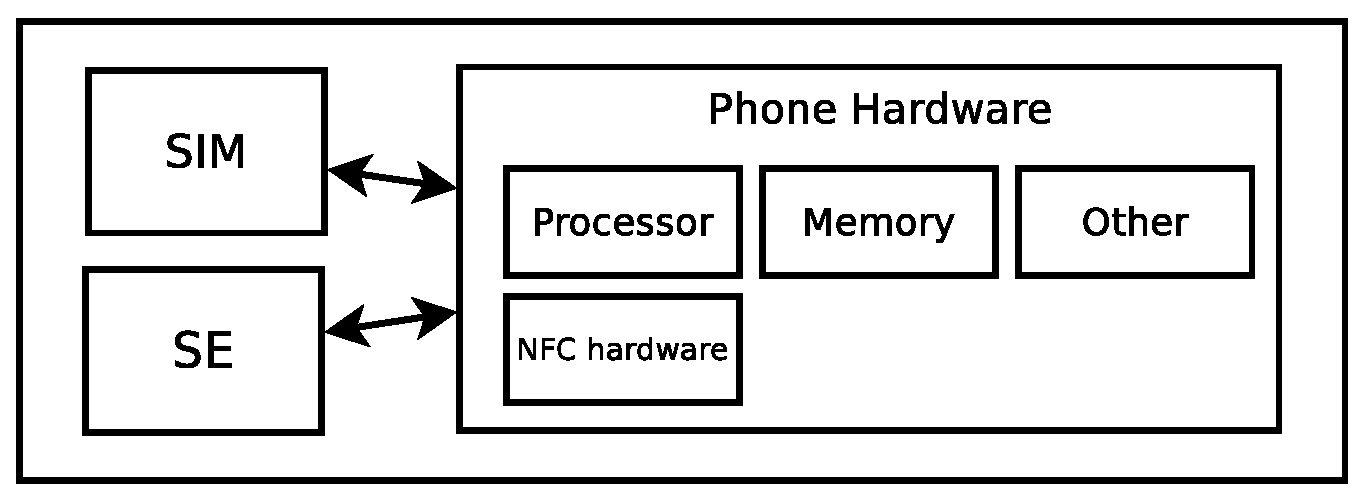
\includegraphics{phone_with_SE_nokia.eps}


Nokia released a phone (Nokia 6131 NFC) in 2006 with NFC as a feature. The architecture of this phone consists of a SIM card, antenna and a seperate Secure Element. The same layout of this architecture can also be used in other mobile devices, see \textit{figure xx}. The phone hardware consists of the usual (processor, memory), but also hardware to provide for NFC features and a secure element to enable payment and ticketing. The secure element stores sensitive data and enables tag and smart card emulation. In case of the Nokia phone it is divided in two subcomponents, a Java Card, used for payment, and Mifare 4k, used for ticketing.

%security problems for this architecture:

An option similar to the Nokia one, is an external SD-card which houses all the hardware needed to enable NFC and also the secure element, see \textit{figure xx}.( http://www.nearfieldcommunicationsworld.com/2009/01/12/3485/tyfone-puts-nfc-into-microsd-cards/)
In this option a third party, e.g. a bank, can issue a SD card to it's customers so they can use the service offered by the bank. 

%security problems for this architecture: SD card might get stolen and used by somebody else.

Related to the above architecture, is the one in \textit{figure xx}. Here the architecture consist of a phone with multiple SIM cards and the usual hardware. In this case a telecom provider will own one SIM card and a bank or public transport company will own the other. This way there no problem with splitting the resources of one SIM card and the trust issue between different companies.

%hier moet nog een bron voor gevonden worden
%security problems for this architecture: SIM card might get stolen and used by somebody else

Of course the option of splitting the resources is also possible, if different companies can find an agreement to share the same SIM card. This is possible, because smartcards in general are becoming more powerfull. This makes two different architectures possible. The first one, see \textit{figure xx}, uses the SIM card as secure element. A phone will have the usual hardware, hardware making NFC possible and SIM card with applications from the telecom provider and applications from a company chosen by the user, e.g. a bank for payment and a public transport company. 
The second option resembles a combination of the first one and the one with the SD card architecture. Here a SIM card has all the hardware needed to make NFC possible and it also acts as a secure element, see \textit{figure xx}. Like the first option, the resources of the SIM card will be split among the involved parties.

%hier moet nog een bron voor gevonden worden
%security problems for this architecture: SIM card might get stolen and used by somebody else





% TODO hoort bij Wireless communication, terwijl 3.2 (Secure Elements) heel ergens anders over gaat
\section{Standardization}
NFC has been described by NFCIP-1 (Near Field Communication Interface Protocol 1) first on ISO18092, ECMA340 and ETSI TS102 and also NFCIP-2 defined in ISO 21481, ECMA352 and ETSI TS102 312.
With NFCIP-2, NFC became compliant with the RFID standards of ISO14443 and ISO15693.

\section{Limitations}

% Toetsenbord en display feature (semi-trusted terminal, moeilijker te tamperen)

% Voorbeeld telefoon met gewone sim en NFC SD card adapter
% Bankier kan heir apps op installeren

% Voorbeeld telefoon met meerdere sims

% Vorobeeld SIM en losse SE, met trusted code

% Voorbeeld SIM van KPN, met apps van de bank

% Uitzoeken:
% Rabomobiel - SIM vd rabobank


%ERIK: figuren toevoegen van verschillende telefoon architecturen. 

% SIM ---> telefoon		SIM = secure, tamper-resitent, authenticatie van telefoon aan het netwerk	marketing redenen (onderscheid welke onderdelen van wie zijn) SIM is van de telco
% a SIM ---> telefoon ---> SE 	SmartMX contactless smartcard  (nokia)
% b SD kaart als a maar vervangbaar SE
% c NFC-SIM